\documentclass[titlepage]{article}
\usepackage{amsmath}
\usepackage{enumerate}
\usepackage{listings}
\usepackage{graphicx}
\title{CS 180 Homework 5}
\author{Robert Geil \\
University of California, Los Angeles
}
\lstset{frame=tb,
  showstringspaces=false,
  columns=flexible,
  basicstyle={\small\ttfamily},
  breaklines=true,
  tabsize=2
}
\numberwithin{equation}{subsection}
\begin{document}
\section{Closest Pair of Points}
\subsection{Problem}
Given a set of $n$ points on a plane, find the closest pair of points, defined by the euclidian distance
between the two
\subsection{Algorithm}
\begin{lstlisting}
1. Sort the input based on x coordinates
2. Split into subgroups of size 2, take the distance between these two to be the shortest
3. For each pair of neighboring subgroups, it must be true that the shortest pair is either the shortest pair on the left, or the shortest pair on the right or a pair containing a single point on left and right
4. Take the minimum of the distances on the left and the right as a value d
5. For each element on the left within that distance d from the split, examine all points on the other side that are also within d in the x direction and either -d or d away from the y coordinate. Save the minimum
6. Take the minimum of the value on the left, the right, and the middle values examined. Set that to be the new min and merge the left and right together
7. If there are still multiple partitions, go to step 3
\end{lstlisting}
\subsection{Proof}
We will prove the correctness by induction. First, for the base case, it is trivially true that for a group of
two points, the shortest path is between those two points, as no other pairing is possible. Inductively, for two
neighboring sets of points, it must be true that the shortest pair is either the shortest pair on the left, or
the shortest pair on the right, or a pair of points where one exists on the left and one on the right. We can see
this is true, as this forms an exhaustive search of all possible points. Finally, we prove that our trick of
only looking at points a distance\textit{delta} from the divide doesn't reject shorter pairs. \textit{delta} is the minimum of the
shortest distances on the left and right. If we look at a pairing of any element on the left (without loss of 
generality) with one on the right, where the left side is more than \textit{delta} away, the distance from left to the 
divide will already be \textit{delta}, and as such the total distance must be \textit{delta} or more. As we already have a pair
satisfying a distance of \textit{delta}, this won't produce a shorter path. Likewise when observing the values above and
below (in the Y direction), we can restrict our search space with the same logic. Any value more than \textit{delta} 
away in the Y direction must already be greater than the min of the shortest distance on the left and right.
Therefore we prove by induction that this algorithm will always find the shortest pair of points.
\subsection{Runtime}
Overall the runtime of this algorithm is O($n\log n$). Initially we perform a sort based on x axis, which takes
O($n\log n$) time. After that, we see that there is a process of dividing and joining into subgroups. Because 
each subgroup is split and joined in a binary fashion, with the same logic as Merge Sort, we see that there 
are O($\log n$) of these join operations. As for the time complexity of each individual operation, we can prove that
each step is done in linear time. Comparing the two existing shortest values on the left and right takes constant
time. To find the pairing across the divide, it would naievely appear that it takes O($n^{2}$) time. However, using
clever constraints, we can reduce this to linear time. First, we select each point on the left that is within
a distance \textit{delta} of the divide. Note this may be O($n$) elements. For each of these, we need only examine
those a distance \textit{delta} from the side, and a distance \textit{delta} above and below the Y coordinate, as
proven above. While this may seem to take linear time to the number of points on the right, we can prove it is
a constant time operation. We claim there are at most a constant number points on the left that must be tested. 
Within the bounding box of \textit{delta} on X and \textit{delta} on Y, the sides can be divided to form grids
that are \textit{delta}/2 by \textit{delta}/2 in size, of which there will be 8. By the pigeonhole principle,
there cannot be more than 1 point within any one of these given boxes. By contradiction, if there were two points
within one box, they would have to be closer than \textit{delta} apart, and would therefore be the shortest on the
right, violating our earlier assumption that \textit{delta} is the shortest distance on the right and left individually.
Therefore, we prove we must only examine a constant number of elements for each element on the left. The searching
of these bounding boxes can be cleverly done with a pre-sorting, by additionally sorting the Y axis points, another
O($n\log n$) task at the beginning. This means each step in the merging takes O($n$) time. Combined over all the
merge steps, we prove we have a final time complexity of O($n\log n$).
\section{Longest Path in Ordered Graph}
\subsection{Problem}
An ordered graph is a DAG such that there is a distinct ordering of nodes by index. Each edge only goes
from a node of a lower index to one of a higher index, and every node besides the last has at least one
edge originating from it. Find the longest path in terms of segment count from node $v_0$ to $v_n$.
\subsection{A Bad Approach}
The provided algorithm is a greedy approach to solving the problem, and it fails under certain situations.
For example, if the first step can pick a nearby value, this will always be added to the solution. However,
due to the greedy nature of the algorithm this may pigeonhole the solution to including a poor choice which
may then jump directly to the end. 
\begin{figure}
    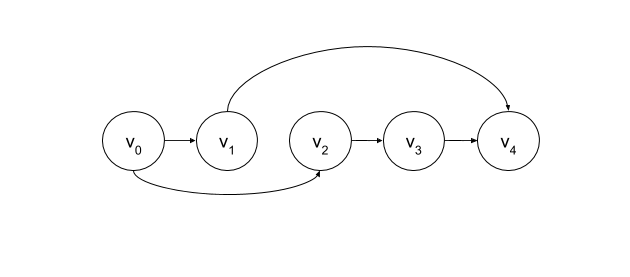
\includegraphics[width=\linewidth]{counter2.png}
    \figurename{: Greedy Counter Example}
\end{figure}
\\
In the above figure, the greedy algorithm would select the path ($v_0$, $v_1$, $v_4$), for a total length of
2 segments. However, the optimal solution is ($v_0$, $v_2$, $v_3$, $v_4$) for a total length of 3 segments.
\subsection{Correct Algorithm}
%TODO
\end{document}